\section{Views}
\label{undirkafli:views}
\section{Yfirlit yfir helstu gagnagrunnskerfi}
\label{undirkafli:helstu-gagnagrunnskerfi}
Gríðarmörg SQL-gagnagrunnskerfi eru til. Í þessum undirkafla verða þau gagnagrunnskerfi sem höfundur telur líklegast að nemendur Tækniskólans muni rekast á í náinni framtíð kynnt.

Grundvallaratriði SQL, sem farið er yfir í þessari bók, hafa miðast við notkun MySQL (\ref{undirkafli:mysql}). Hugmyndirnar á bak við þessi grundvallaratriði er sú sama í öllum gagnagrunnskerfum sem byggja á SQL, en \emph{útfærslan} er ekki endilega sú sama. Við skulum ekki búast við því að sýnidæmi bókarinnar keyri óbreytt í öllum gagnagrunnskerfum.
\subsection{MySQL}
\label{undirkafli:mysql}
\begin{marginfigure}
\caption{MySQL}
\label{mynd:mysql}
\centering

\includegraphics[width=\linewidth]{myndir/mysql}
\end{marginfigure}
MySQL\footnote{\url{http://www.mysql.com/}} er gagnagrunnskerfi í mikilli notkun, sérstaklega við vefsíðugerð.

Þökk sé útbreiðslunni er tiltölulega auðvelt að finna leiðbeiningar um notkun MySQL og uppsetningu MySQL-servera. Hægt er að vinna með MySQL í gegnum fjölmörg forritunarmál. MySQL er opið\footnote{e. \emph{open source}} og ókeypis.

MySQL hefur skilist að í nokkra hluta síðan það var fyrst gefið út. Upprunalegir höfundar kerfisins vinna nú við afbrigði sem heitir MariaDB\footnote{\url{https://mariadb.org/}}.
\subsection{PostgreSQL}
\begin{marginfigure}
\caption{PostgreSQL}
\label{mynd:postgresql}
\centering

\includegraphics[width=0.8\linewidth]{myndir/postgresql}
\end{marginfigure}
PostgreSQL\footnote{\url{http://www.postgresql.org/}} er gagnagrunnskerfi sem leggur mikla áherslu á að fylgja stöðlum og bjóða upp á ``rétta'' gagnavinnslu.

PostgreSQL er vinsælt meðal gagnagrunnssérfræðinga, m.a. vegna þess hversu mikla stjórn gagnagrunnstjórinn hefur yfir virkni kerfisins. Kennt er á PostgreSQL gagnasafnsfræðiáföngum Tækniskólans.

Fyrir utan það að styðja ``venjulegar'' SQL skipanir, þá býður PostgreSQL upp á forritunarmál, kallað PL/pgSQL (Procedural Language/PostgreSQL), til að auðvelda ýmsar aðgerðir. PL/pgSQL býður meðal annars upp á lykkjur og önnur tól sem kunnugleg eru úr forritunarmálum á borð við C\#.
\subsection{SQLite}
\begin{marginfigure}
\caption{SQLite}
\label{mynd:sqlite}
\centering

\includegraphics[width=\linewidth]{myndir/sqlite}
\end{marginfigure}
SQLite\footnote{\url{http://sqlite.org/}} er ólíkt flestum gagnagrunnskerfum að því leyti að ekki þarf að setja upp eiginlegt kerfi á tölvunni sem á að hýsa gagnagrunninn, allt forritið er ein skrá.

Smæðarinnar vegna vantar SQLite ýmsa eiginleika sem stærri gagnagrunnskerfi bjóða upp á, en það hentar sérstaklega vel til að nota sem hluta af stærri kerfum. SQLite má finna ``undir húddinu'' á mörgum forritum sem þurfa að geyma gögn.
\subsection{Microsoft SQL Server}
\begin{marginfigure}
\caption{SQL Server}
\label{mynd:sql-server}
\centering
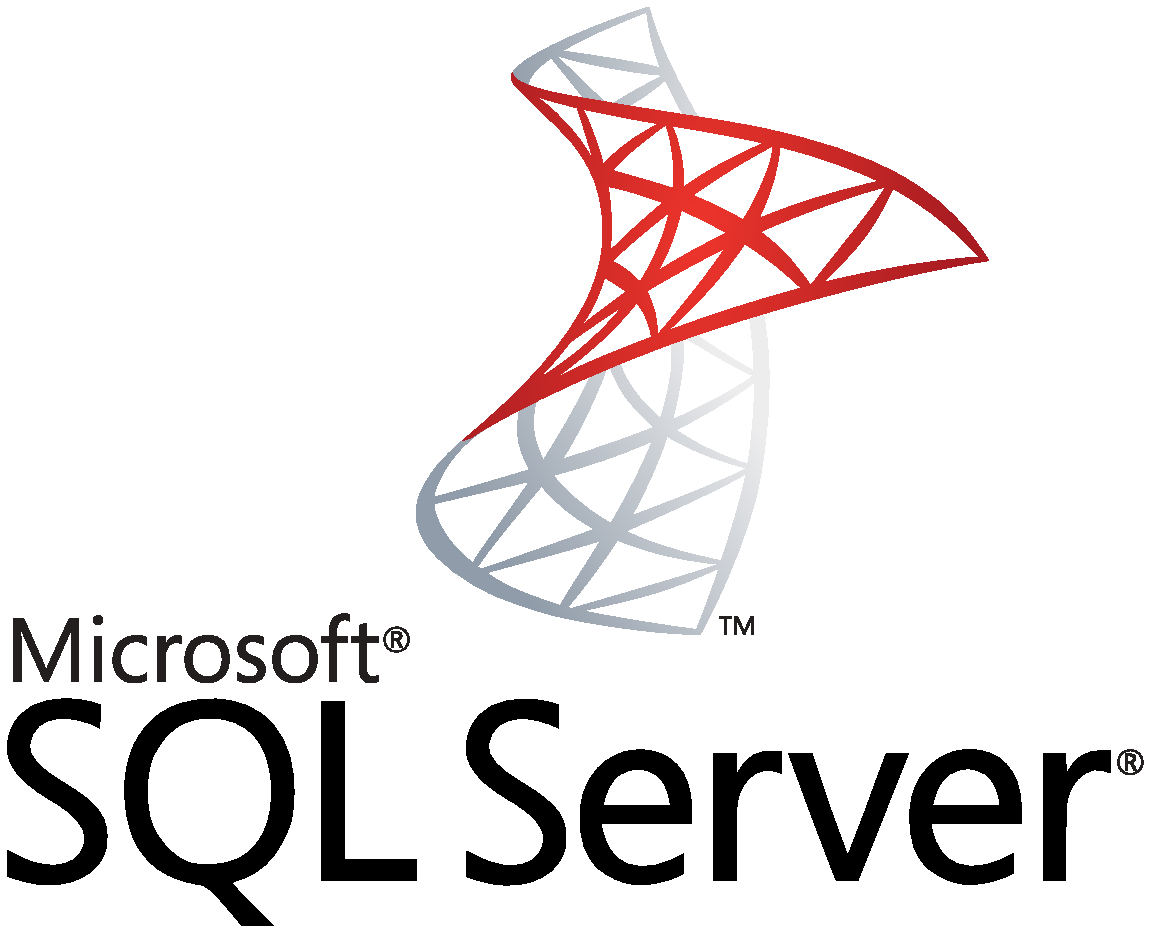
\includegraphics[width=\linewidth]{myndir/sql-server}
\end{marginfigure}
SQL Server\footnote{\url{http://www.microsoft.com/sqlserver}} er gagnagrunnskerfi gefið út af Microsoft. Það er sniðið til að passa vel til keyrslu á Windows-vélum. SQL Server er helsti keppinautur Oracle gagnagrunnskerfisins þegar kemur að stórum gagnagrunnum.

Sú útgáfa af SQL sem notuð er til samskipta við SQL Server heitir Transact-SQL. T-SQL styður lykkjur og breytur.
\subsection{Oracle Database}
\label{undirkafli:oracle}
\begin{marginfigure}
\caption{Oracle Database}
\label{mynd:oracle}
\centering

\includegraphics[width=\linewidth]{myndir/oracle}
\end{marginfigure}
Gagnagrunnskerfi Oracle\footnote{\url{http://www.oracle.com/us/products/database/overview/}} er mest notaða gagnagrunnskerfi í heimi í dag. Það hefur verið í þróun áratugum saman og knýr marga af heimsins stærstu gagnagrunnum.

Útvíkkun Oracle á SQL til að styðja lykkjur og önnur algeng forritunaratriði er kallað PL/SQL (Procedural Language/Structured Query Language).
\section{Venslalíkanið}
SQL byggir á föstum stærðfræðilegum grunni. Sá grunnur er kallaður \emph{venslalíkanið}\footnote{e. \emph{Relational model}}. Því var fyrst lýst af tölvunarfræðingnum Edgar Codd um 1970\footnote{Aðalgreinin sem lýsir því heitir ``\emph{A Relational Model of Data for Large Shared Data Banks}''. Áhugasamir geta fundið hana á netinu.}.

Venslalíkanið lýsir því hvernig líta má á gögn sem stök í mengjum og hvernig nota má þekktar\footnote{Þær eru í það minnsta þekktar flestum stærðfræðingum.} stærðfræðiaðgerðir til að nálgast þær. 

SQL er \emph{útfærsla} á venslalíkaninu. Uppbygging þess leiðir til þess að þegar við tölum um SQL notum við sjaldnast sama orðaforða og er notaður í stærðfræðinni sem það byggir á. Engu að síður er skilningur á venslalíkaninu og þeim orðaforða sem þar kemur við sögu mjög gagnlegur öllum sem nota SQL.

Ítarleg umfjöllun um venslalíkanið er viðfangsefni fyrir háskólanámskeið, ekki þessa bók. Engu að síður skulum við skoða mikilvægasta hugtak líkansins, \emph{vensl}, og hvernig það passar við það sem við höfum séð af SQL í þessari bók.
\subsection{Mengi}
Áður en lengra er haldið skulum við vera viss um að við höfum hugmynd um hvað \emph{mengi}\footnote{e. \emph{set}} er. Þetta eru sömu mengin og við höfum kynnst í grunnskólastærðfræði.

Mengi er safn/hópur af fyrirbærum. ``Fyrirbærin'' í mengi geta verið nær hvað sem er, t.d. tölur, orð, eða önnur mengi. ``Heiltölur'', ``Íslendingar'' og ``Rauðir hlutir'' eru allt mengi.

Tvö atriði einkenna mengi:
\begin{itemize}
 \item Röð hluta í mengi skiptir ekki máli.
 \item Aldrei er um endurtekningar að ræða í mengi. Hlutur er annaðhvort í mengi eða hann er það ekki.
\end{itemize}
Þegar hlutur er í mengi er talað um að hluturinn sé \emph{stak} í menginu.

Mengjum er oft gefið nafn sem er einn stór bókstafur. T.d. er algengt að kalla mengi heiltalna $N$. 

Þetta gerir okkur mögulegt að kynnast fleiri hugtökum. Skoðum tvö mengi, $A$ og $B$. Það skiptir okkur ekki máli hvað er í mengjunum.
\begin{itemize}
 \item Séu öll stök í mengi $A$ líka stök í mengi $B$ er sagt að $A$ sé \emph{hlutmengi} $B$.
 \item Séu einhver stök í mengi $A$ sem líka eru í mengi $B$ er sagt að þau stök séu í \emph{sniðmengi} $A$ og $B$.
 \item Mengi sem inniheldur öll stök úr mengjum $A$ og $B$ er kallað \emph{sammengi} $A$ og $B$.
\end{itemize}


\subsection{Vensl}
Við skulum sjá fyrir okkur mörg mengi af upplýsingum. Köllum þau öll $S$ og gefum þeim númer, svo við getum kallað þau $S_1, S_2$ og svo framvegis.

Skoðum nú annað mengi og köllum það $R$. Mengið $R$ er \emph{vensl\footnote{e. \emph{relation}} á mengin $S$} ef $R$ er mengi af \emph{línum}\footnote{e. \emph{tuples}} þar sem að fyrsta gildið í línunni er úr $S_1$, annað stakið úr $S_2$, og svo framvegis.

Til að gera venslin nothæf getum við ákveðið að hvert mengi $S$ standi fyrir einhvern ákveðinn \emph{eiginleika}\footnote{e. \emph{attribute}} sem gögn geta haft. Þá stendur hver lína í venslunum fyrir einn ``hlut'' sem einkennist af þeim eiginleikum sem við skilgreindum.

Hvernig tengist þetta þeim hugtökum sem við höfum lært úr SQL?

\begin{itemize}
 \item Lína í SQL-töflu samsvarar (e. \emph{tuple}) í venslum.
 \item Dálkur í SQL-töflu samsvarar eiginleika (e. \emph{attribute}) í venslum.
 \item SQL-tafla samsvarar að mestu leyti venslum.\footnote{Vensl og SQL-töflur greinast að á nokkrum atriðum. T.d. eru vensl alvöru mengi, sem ekki geta verið með endurtekningar. SQL-tafla sem ekki er með aðallykil getur innihaldið endurtekin gildi.}
 \item Niðurstöður fyrirspurna og view-a (sjá undirkafla \ref{undirkafli:views}) samsvara líka að mestu leiti venslum.
\end{itemize}

Það að skilja venslalíkanið gerir sum atriði sem viðkoma SQL skýrari, t.d. samband view-a og taflna. Einnig getum við nú séð að þegar rætt er um venslaðar töflur er átt við töflur sem hægt er að búa til vensl á.


\section{Að tengjast gagnagrunni með PHP}
\label{undirkafli:php}
Við höfum eytt miklum tíma í að skoða gagnagrunna sem sjálfstætt fyrirbrigði.

Í þessum undirkafla skoðum við loksins hvernig tengja má MySQL-gagnagrunn við PHP-forritskóða.
Slíkar tengingar eru teknar fyrir vegna þess hve algengar\footnote{Linux, Apache, PHP og MySQL mynda saman ``pakka'' sem oft er notaður sem ein heild. Pakkinn er nefndur eftir skammstöfun sinni, LAMP. Hann er í gríðarmikilli notkun.} þær eru í vefforritun.

Útskýringarnar gera ráð fyrir skilningi á ýmsum atriðum:
\begin{itemize}
 \item Hugtökum í vefsíðum - HTML, Javascript
 \item Keyrslu PHP-skripta
 \item Grundvallarmálfræði PHP
 \item IP-tölum
 \item Föllum, lykkjum og fylkjum\footnote{e. \emph{functions}, \emph{loops} og \emph{arrays}}
\end{itemize}
\subsection{Hlutverk gagnagrunna í vefsíðum}
Vefsíða sem byggð er upp á hefðbundinn hátt skiptist gróflega í tvo hluta - client og server. 

\begin{figure}
\centering
\caption{Hefðbundin uppbygging vefsíðu}
\label{mynd:uppbyggingvefsidu}
\color{red} Hingað kemur falleg mynd af client-server strúktúr vefsíðu.
\end{figure}

Client-hlutinn er sá hluti sem keyrður er á tölvu notandans. Í client-hluta eru HTML-tög túlkuð og Javascript-kóði keyrður, m.a.. Venjulega fer þessi vinna fram í vafra\footnote{e. \emph{browser}, t.d. Google Chrome, Firefox og Internet Explorer} notandans.

Server-hlutinn er margskiptur. Viðfangsefni okkar, PHP og MySQL, tilheyra þessum hluta. Oft keyra PHP og MySQL á sömu tölvu, sem er þá einfaldlega nefnd ``serverinn''.

Hlutverk gagnagrunnsins í þessari uppbyggingu er, eðli hans samkvæmt, það að halda utan um upplýsingar. PHP-hluti serversins sér um að eiga samskipti við gagnagrunninn og miðla upplýsingunum áfram til clientsins. Notandinn og tölva hans eiga aldrei bein samskipti við MySQL-serverinn.

\subsection{Uppsetning tengingar með PDO}
Gerum ráð fyrir að við séum með PHP-skriptu sem keyrir á vefþjóni. Til að tengjast MySQL-gagnagrunni þarf hún eftirfarandi upplýsingar:
\begin{itemize}
 \item Tengingarupplýsingar: Gagnagrunnsgerðina (hjá okkur alltaf MySQL), nafn gagnagrunnsins og staðsetningu hans
 \item Notandanafn MySQL-þjónsins
 \item Lykilorð notandans.
\end{itemize}
Klasann \href{http://www.php.net/manual/en/class.pdo.php}{PDO}\footnote{\url{http://www.php.net/manual/en/class.pdo.php}} má svo nota til þess að mynda tenginguna sjálfa.\footnote{Fleiri leiðir eru færar til að mynda tengingar af þessum toga, til dæmis \emph{mysqli} viðbótin. Þá PHP-viðbót sem einfaldlega heitir \emph{mysql} skal þó alls ekki nota - hún er úreld.}

\begin{example}[h]
\caption{Tenging við gagnagrunn með PDO}
\label{sql:k8d1}
\centering
\inputminted[frame=lines, fontfamily=courier]{php}{php/k8d1.php}
\end{example}

Dæmi um hvernig öll skriptan gæti litið út má sjá á sýnidæmi \ref{sql:k8d1}. Skoðum það sýnidæmi nánar. 

Fyrsta breytan sem er skilgreind í skriptunni (\verb|$source|) inniheldur tengingarupplýsingarnar. Þar kemur fyrst fram orðið \verb|mysql|, aðskilið frá gagnagrunnsnafninu og staðsetningu gagnagrunnins með tvípunkti. Sé ætlunin að skrifa skriptu af þessum toga til nota í eigin forriti þyrfti að skipta út \verb|testdb| fyrir nafn gagnagrunnsins sem nota skal. Sé MySQL-serverinn ekki að keyra á sömu tölvu og PHP-skriptan þarf einnig að breyta IP-tölunni í IP-tölu tölvunnar sem MySQL-serverinn keyrir á.\footnote{Server Upplýsingatækniskólans keyrir á IP-tölunni \emph{82.148.66.15}. Einnig má skrifa nafn hans, \emph{tsuts.tskoli.is}, í stað IP-tölunnar.}

Næstu tvær breytur innihalda notandanafn og lykilorð fyrir MySQL-serverinn. Þetta er sama notandanafn og lykilorð og notað var til að tengjast gagnagrunninum í kafla \ref{kafli:fyrstuskrefin}.

Þegar upplýsingarnar hafa verið geymdar er loks ``reynt'' að búa til tengingu með PDO. Takist það eru tengingarupplýsingarnar geymdar í  ``database handle'' breytu, nefnd \verb|$dbh| í sýnidæminu. Þessa breytu má síðan nýta til að eiga samskipti við gagnagrunninn.

Takist ekki að koma tengingunni á prentar skriptan út strenginn ``Tenging mistókst'' ásamt villuskilaboðunum sem berast.
\subsection{Að sækja gögn með PDO}
\subsection{Að birta gögn á vefsíðu}